\documentclass[PhD-Yoann-Dupont.tex]{subfiles}
\begin{document}

Récemment, le domaine du TAL a vu un essor des réseaux de neurones \emph{récurrents}. Ces derniers ont été créés pour traiter des séquences de données selon un principe simple : pour chaque élément d'une séquence, son résultat est injecté dans l'élément suivant de la séquence, permettant ainsi, de proche en proche, d'incorporer le contexte à un instant donné. Le réseau récurrent le plus simple étant le réseau d'Elman \citep{elman1990finding}, où la couche cachée d'un réseau communique avec elle-même, à l'instar des n\oe uds dans une liste chaînée. Cependant, ces derniers n'arrivaient pas à modéliser des dépendances longue distance et leur apprentissage était très coûteux \citep{bengio1994learning}.

La couche cachée \emph{Long Short-Term Memory} \citep{hochreiter1997long}, appelée par la suite LSTM, s'est distinguée par sa capacité à capturer des dépendances de longue portée, palliant deux problèmes liés à la propagation à travers le temps lors de l'entrainement d'un RNN classique. Ces deux problèmes analogues sont l'extinction et l'explosion du gradient \citep{hochreiter1997long}. Ces deux phénomènes surviennent lors de l'actualisation des poids par rétropropagation. On parle d'extinction du gradient lorsque les valeurs du gradient tendent exponentiellement vers 0, la mise à jour des poids dans le réseau étant alors très faible. Le RNN a en conséquence du mal à sortir d'une configuration locale, le coût en temps de son apprentissage devient prohibitif. L'explosion du gradient est un phénomène analogue dans lequel les valeurs croissent de façon exponentielle. Cela provoque un phénomène d'oscillation des poids, qui prennent des valeurs extrêmes d'une mise à jour à l'autre. Cela rend très complexe la convergence vers un extremum local, l'oscillation des valeurs étant trop importante pour converger. LSTM est un type particulier de couche cachée dans un réseau d'Elman. La figure\ \ref{fig:lstm-cell} illustre le fonctionnement d'une cellule d'une couche cachée LSTM, elle est l'équivalent du "R" dans la figure\ \ref{fig:FFNN-vs-RNN}.


\begin{figure}[ht!]
\centering
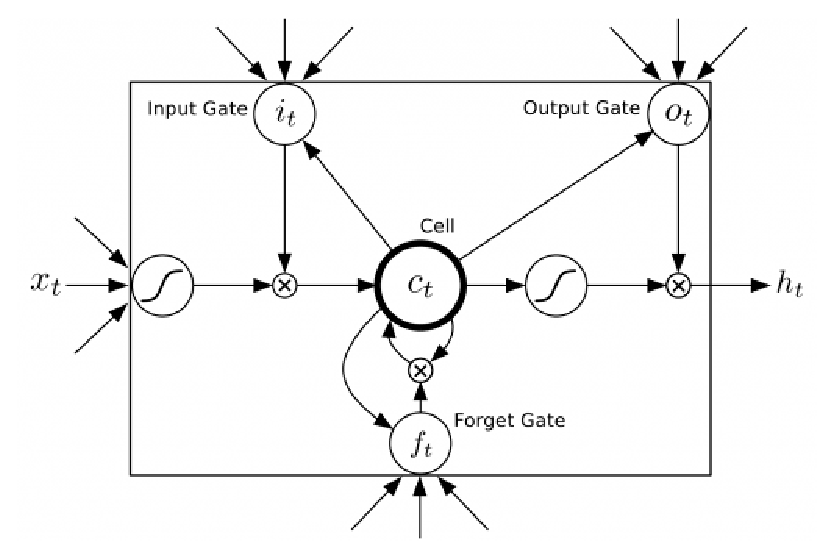
\includegraphics[scale=0.75]{images/LSTM/LSTM-cell}
\caption{une cellule dans un LSTM}
\label{fig:lstm-cell}
\end{figure}

Le principe d'un LSTM réside dans le fait que le réseau dispose d'une mémoire et va de lui-même apprendre à ne conserver que les valeurs intéressantes via un mécanisme de portes illustré dans la figure \ref{fig:lstm-cell}, cette dernière permettant de compenser les deux problèmes du gradient en donnant au réseau une forme de stabilité. L'état courant est représenté par la cellule $c[t]$. Un LSTM dispose de trois portes : la porte d'entrée ($i[t]$), d'oubli ($f[t]$) et de sortie ($o[t]$). La porte d'entrée permet de récupérer les informations pertinentes à conserver en mémoire dans l'état courant, celle d'oubli permet d'en retirer des informations qui ne sont plus pertinentes. Une fois modifié, l'état courant est combiné avec la porte de sortie pour créer la couche cachée qui servira d'entrée à la cellule suivante dans le réseau, dont les formules respectives sont données dans les équations \ref{eq:lstm}.

\begin{equation}\label{eq:lstm}
\begin{aligned}
f_{t}     &= \sigma(W_{f} \times h_{t-1} + U_{f} \times I_{t} + b_{f}) \\
i_{t}     &= \sigma(W_{i} \times h_{t-1} + U_{i} \times I_{t} + b_{i}) \\
\hat{c}_t &= tanh(W_{c} \times h_{t-1} + U_{c} \times x_{t} + b_c) \\
c_{t}     &= f_{t} \odot c_{t-1} + i_{t} \odot \hat{c}_{t} \\
o_{t}     &= \sigma(W_{o} \times h_{t-1} + U_{o} \times I_{t} + b_{o}) \\
h_{t}     &= o_{t} \odot \sigma(c_{t})
\end{aligned}
\end{equation}

Les LSTM sont des variantes de réseaux d'Elman dont le principe peut se résumer à un raffinement de la couche cachée. Cette piste est particulièrement explorée dans le TAL, où de variantes de la LSTM sont proposées \citep{chung2014empirical,greff2015lstm,zaremba2015empirical}, la plus connue étant la \emph{Gated Recurrent Unit}, ou GRU \citep{cho2014properties}. Ce réseau peut se voir comme une simplification de la LSTM, où les portes d'entrée et d'oubli sont fusionnées en une porte de mise-à-jour, ainsi que la cellule et la couche cachée précédente. Ces réseaux ont montré des performances similaires aux LSTM tout en étant plus simple d'un point de vue computationel, ce qui les rend plus intéressants. Une autre piste de recherche dans le domaine des réseaux récurrents consiste à non pas raffiner mais étendre les réseaux de Elman. Dans la prochaine section, nous détaillerons ces réseaux.

\end{document}